\chapter{Exploration}

\section{Slice}

\textbf{Énoncé} : Effectuez une requête simple afin de déterminer le montant total des ventes pour l’année 2008.

\begin{figure}[H]
\centering
\begin{lstlisting}
select [Dim.Date].[Dim.Date.ByMonth].[Year].[2008] on rows,
[Measures].[SalesAmount] on columns from [AdventureCube]
\end{lstlisting}
\caption{Requête Slice : montant total des ventes pour l'année 2008}
\label{lst:reqSlice}
\end{figure}

\begin{figure}[H]
    \centering
    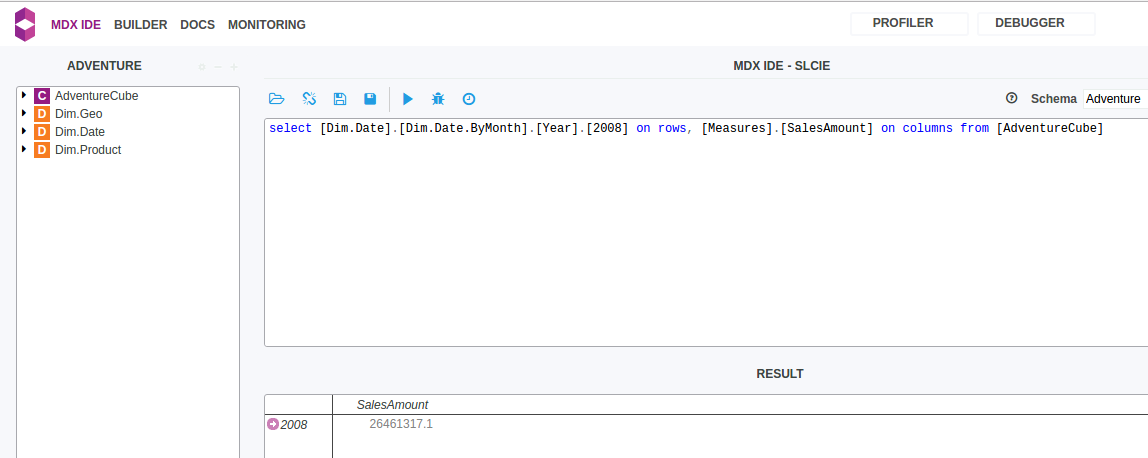
\includegraphics[width=1\linewidth, fbox]{img/requeteSlice.png}
    \caption{Résultat requête Slice : montant total des ventes pour l'année 2008}
    \label{reqSliceResult}
\end{figure}

Le résultat obtenu est : 26461317.1

\pagebreak

\section{Dice}

\textbf{Énoncé} : Déterminer le montant des ventes de l’article « Fender Set – Mountain » pour l’année 2008 en Californie. [Accessoires -> Fenders -> Fender Set – Mountain]

\begin{figure}[H]
\centering
\begin{lstlisting}
select [Dim.Date].[Dim.Date.ByMonth].[Year].[2008] on rows,
	   [Measures].[SalesAmount] on columns
from [AdventureCube]
where (
	   [Dim.Geo].[Dim.Geo].[Country].[United States].[California],
	   [Dim.Product].[Dim.Product].[Product].&[485]
      )
\end{lstlisting}
\caption{Requête Dice : montant des ventes de l'article « Fender Set – Mountain » pour l'année 2008}
\label{lst:reqDice}
\end{figure}

\begin{figure}[H]
    \centering
    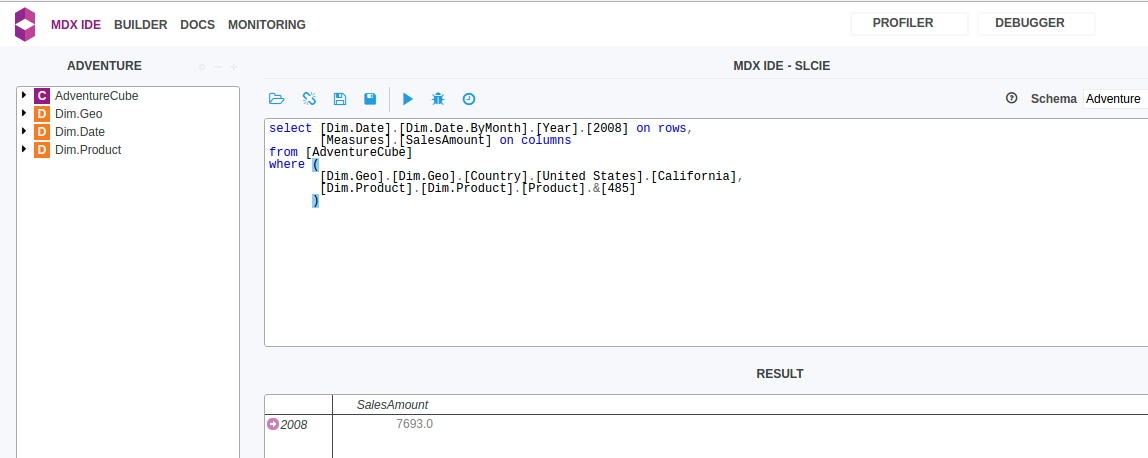
\includegraphics[width=1\linewidth, fbox]{img/requeteDice.png}
    \caption{Résultat requête Dice : montant des ventes de l'article « Fender Set – Mountain » pour l'année 2008}
    \label{reqSliceDice}
\end{figure}

Le résultat obtenu est : 7693

\pagebreak

\section{Roll-up}

\textbf{Énoncé} : En utilisant le principe du Roll-up, déterminez le montant des ventes de l’article « Fender Set – Mountain » pour l’ensemble des États-Unis ainsi que pour l’ensemble des pays, toujours pour l’année 2008.

\subsubsection*{Étas-Unis}

\begin{figure}[H]
\centering
\begin{lstlisting}
select ([Dim.Geo].[Country].[United States], [Dim.Product].[Product].&[485]) on columns,
[Measures].[SalesAmount] on rows
from [AdventureCube]
where [Dim.Date].[Dim.Date.ByMonth].[Year].[2008]
\end{lstlisting}
\caption{Requête Roll-up : montant des ventes de l'article « Fender Set – Mountain » Étas-Unis en 2008}
\label{lst:reqRollUpUS}
\end{figure}

\begin{figure}[H]
    \centering
    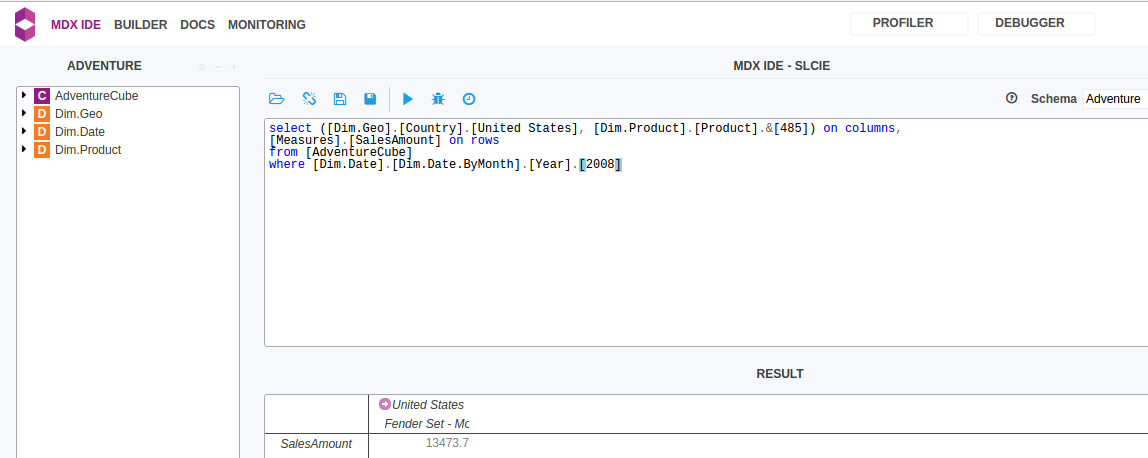
\includegraphics[width=1\linewidth, fbox]{img/requeteRollUpUS.png}
    \caption{Résultat requête Roll-up : montant des ventes de l'article « Fender Set – Mountain » Étas-Unis en 2008}
    \label{reqRollUpResultUS}
\end{figure}

Le résultat obtenu pour les Étas-Unis est : 13473.7

\subsubsection*{Tous les pays}

\begin{figure}[H]
\centering
\begin{lstlisting}
select ([Dim.Geo].[Dim.Geo],[Dim.Product].[Dim.Product].[Product].&[485]) on columns,
[Measures].[SalesAmount] on rows
from [AdventureCube]
where [Dim.Date].[Dim.Date.ByMonth].[Year].[2008]
\end{lstlisting}
\caption{Requête Roll-up : montant des ventes de l'article « Fender Set – Mountain » Étas-Unis en 2008}
\label{lst:reqRollUpUS}
\end{figure}

\begin{figure}[H]
    \centering
    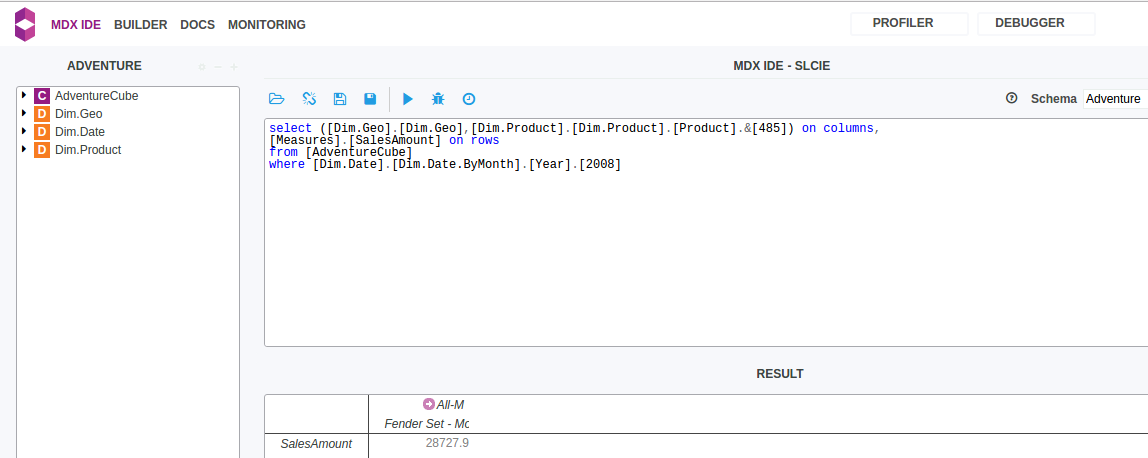
\includegraphics[width=1\linewidth, fbox]{img/requeteRollUpPays.png}
    \caption{Résultat requête Roll-up : montant des ventes de l'article « Fender Set – Mountain » Tous les pays en 2008}
    \label{reqRollUpResultPays}
\end{figure}

Le résultat obtenu pour tous les pays est : 28727.9

\pagebreak

\section{Drill-down}

\textbf{Énoncé} : Pour l’ensemble des pays, déterminez quel trimestre de 2008 a été le plus fructueux au niveau des ventes de l’article « Fender Set – Mountain ». Quel a été le montant total des ventes ?

\subsubsection*{Ordre chronologique}

\begin{figure}[H]
\centering
\begin{lstlisting}
select ([Dim.Geo], [Dim.Product].[Product].&[485]) on rows,
[Dim.Date].[Dim.Date.BySemester].[Quarter] on columns
from [AdventureCube]
where [Dim.Date].[Dim.Date.ByMonth].[Year].[2008]
\end{lstlisting}
\caption{Requête Drill-Down - Chronologique}
\label{lst:reqDrill1}
\end{figure}

\begin{figure}[H]
    \centering
    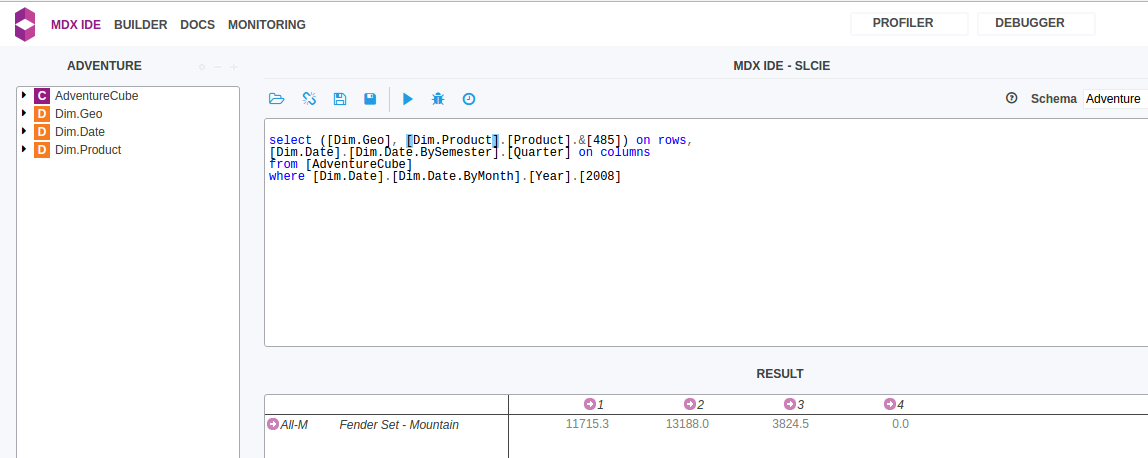
\includegraphics[width=1\linewidth, fbox]{img/requeteDrill1.png}
    \caption{Résultat requête Drill-Down - Chronologique}
    \label{reqDrill1}
\end{figure}

\subsubsection*{Ordre par trimestre le plus fructueux}

\begin{figure}[H]
\centering
\begin{lstlisting}
select ([Dim.Geo], [Dim.Product].[Product].&[485]) on rows,
order([Dim.Date].[Dim.Date.BySemester].[Quarter], [Measures].[SalesAmount], DESC) on columns
from [AdventureCube]
where [Dim.Date].[Dim.Date.ByMonth].[Year].[2008]
\end{lstlisting}
\caption{Requête Drill-Down - Trimestre le plus fructueux}
\label{lst:reqDrill2}
\end{figure}

\begin{figure}[H]
    \centering
    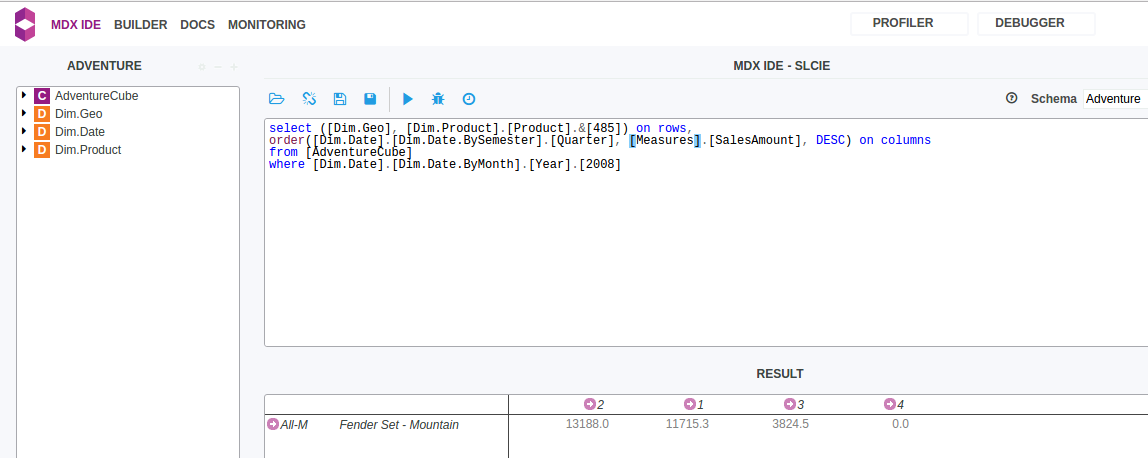
\includegraphics[width=1\linewidth, fbox]{img/requeteDrill2.png}
    \caption{Résultat requête Drill-Down - Trimestre le plus fructueux}
    \label{reqDrill2}
\end{figure}
